\chapter{Estado de la cuestión}

La caracterización acústica de recintos mediante la Respuesta al Impulso de la Sala (RIR) es un desafío complejo que combina aspectos físicos, matemáticos y computacionales. Esta sección sitúa el estado de la cuestión desde los métodos geométricos clásicos (Ray Tracing e ISM), útiles para el análisis físico de salas, hasta los enfoques de aprendizaje profundo orientados a extrapolar la reverberación tardía con mayor eficiencia y capacidad de generalización.

\section[Acústica geométrica]{Acústica geométrica para el análisis de salas y la síntesis de RIR}

\subsection{Trazado de Rayos (\textit{Ray Tracing})}

Introducido en la acústica de salas a finales de la década de 1960 \cite{Krokstad1968}, el trazado de rayos es un método estadístico que discretiza la energía acústica emitida por una fuente omnidireccional o direccional. El algoritmo emite un número finito de rayos que se propagan por el entorno virtual tridimensional. Cada vez que un rayo colisiona con un polígono, su energía disminuye en función del coeficiente de absorción del material, y se refleja de manera especular (siguiendo la ley de Snell) o se dispersa de manera difusa según el coeficiente de \textit{scattering}. Para registrar la respuesta de impulso, se define un volumen de recepción (habitualmente esférico); cuando un rayo atraviesa este volumen, su energía, tiempo de llegada y dirección se acumulan en la Respuesta al Impulso de la Sala (RIR).

A pesar de ser el estándar en la industria para auralización, el trazado de rayos presenta limitaciones matemáticas y computacionales  cuando se trata de sintetizar colas de reverberación densas y largas. Estudios  sobre la optimización de motores de simulación geométrica, como la evaluación del entorno GSound-SIR \cite{Zang2025GSoundSIR}, han cuantificado empíricamente la ineficiencia de este método:

\begin{itemize}
    \item \textbf{Escalabilidad lineal del coste computacional:} El tiempo de simulación y el procesamiento de rutas válidas crecen de manera estrictamente lineal respecto al número total de rayos emitidos \cite{Zang2025GSoundSIR}. Para lograr una densidad suficiente en la reverberación tardía , se requiere proyectar millones de rayos, lo que satura los recursos de procesamiento e imposibilita su uso dinámico en tiempo real.
    \begin{figure}[H]
    \centering
    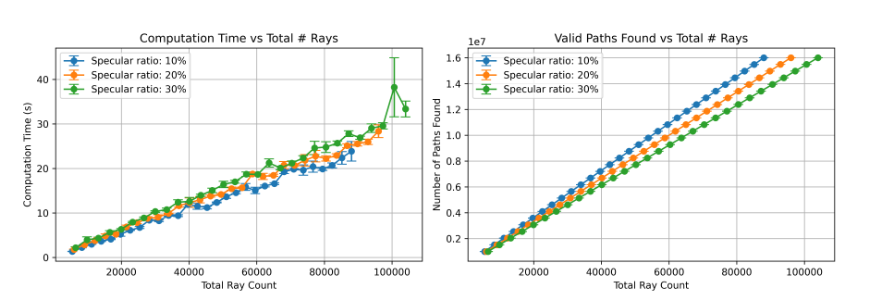
\includegraphics[width=0.75\linewidth]{Figures/gsound_computation_time.png} % Asegúrate de guardar el recorte con este nombre
    \caption[Coste computacional del trazado de rayos]{Relación entre el tiempo de cálculo computacional y el número total de rayos emitidos, categorizado por el porcentaje de rayos especulares. El escalado estrictamente lineal subraya la limitación del método para simulaciones de alta densidad acústica. \cite{Zang2025GSoundSIR}}
    \label{fig:gsound_computation}
\end{figure}
    
    \item \textbf{Sobrecarga por reflexiones especulares:} La validación de trayectorias físicas libres de obstrucciones entre la fuente y el oyente es computacionalmente costosa. Las configuraciones de simulación que exigen un mayor porcentaje de reflexión especular frente a la difusa incrementan exponencialemente el tiempo de cálculo \cite{Zang2025GSoundSIR}.
    
    \begin{figure}[H]
        \centering
        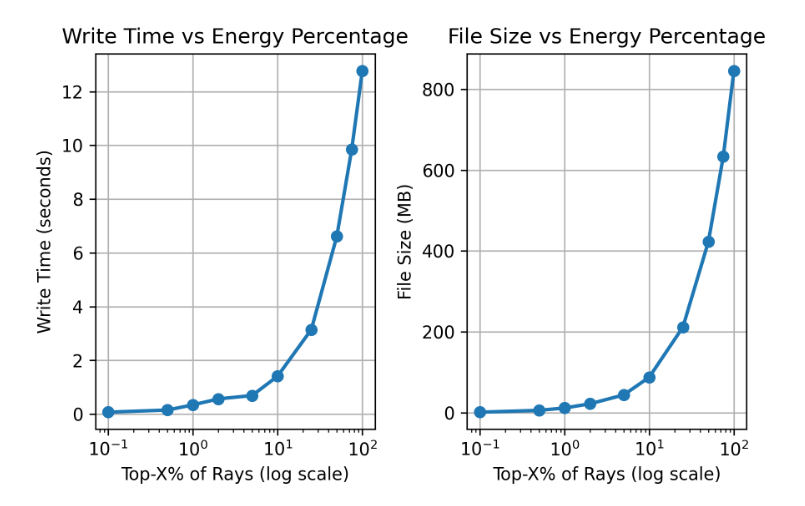
\includegraphics[width=0.85\linewidth]{Figures/gsound_storage_performance.png} % Asegúrate de que el nombre del archivo coincida
        \caption[Rendimiento de almacenamiento según porcentaje de rayos]{Relación entre el tiempo de escritura en disco (izquierda) y el tamaño del archivo resultante (derecha) en función del porcentaje de rayos de mayor energía procesados. Aprovechar la redundancia energética descartando la inmensa mayoría de rayos de baja energía permite un ahorro drástico en los costes de almacenamiento y lectura de la simulación. \cite{Zang2025GSoundSIR}}
        \label{fig:gsound_storage}
    \end{figure}

    
    \item \textbf{Redundancia energética masiva:} El análisis de distribución de energía en simulaciones densas revela que el cálculo exhaustivo de rayos es extremadamente ineficiente. Las mediciones indican que apenas el $0,1\%$ de los rayos capturan el $81,8\%$ de la energía acústica total de la sala, y el $10\%$ superior de los rayos modela el $99,6\%$ de la energía \cite{Zang2025GSoundSIR}. Esto demuestra que los métodos tradicionales invierten la inmensa mayoría de sus ciclos de reloj en trazar decenas de miles de reflexiones tardías que apenas aportan una fracción marginal a la reconstrucción energética de la RIR.
    
    \begin{figure}[H]
    \centering
    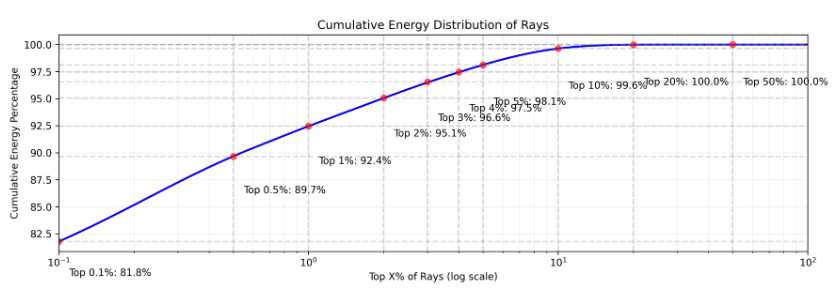
\includegraphics[width=0.75\linewidth]{Figures/gsound_energy_distribution.png} % Asegúrate de guardar el recorte con este nombre
    \caption[Distribución de energía acústica en trazado de rayos]{Distribución de energía acústica acumulada en función del porcentaje de rayos simulados. Se observa que el 10\% de los rayos de mayor intensidad concentran el 99,6\% de la energía total, evidenciando la redundancia del cálculo exhaustivo para la reverberación tardía. \cite{Zang2025GSoundSIR}}
    \label{fig:gsound_energy}
    \end{figure}
    \end{itemize}

Esta redundancia energética y el alto coste computacional asociado a la resolución espacial exhaustiva evidencian el límite tecnológico del \textit{Ray Tracing}. Como sugieren los propios autores del estudio, la enorme concentración de energía en una fracción mínima de rayos abre la puerta a enfoques basados en aprendizaje profundo \cite{Zang2025GSoundSIR}; específicamente, a modelos capaces de reconstruir y extrapolar la respuesta impulsional completa a partir de un conjunto reducido de rayos de alta energía, los cuales corresponden físicamente al campo directo y a las primeras reflexiones \cite{Zang2025GSoundSIR}. 

\subsection{Método de Fuentes Imagen (ISM)}

El Método de Fuentes Imagen (\textit{Image Source Method}, ISM) es una de las técnicas de acústica geométrica más rigurosas para el modelado de reflexiones especulares. Formalizado originalmente por Allen y Berkley en 1979 para recintos de geometría rectangular estricta \cite{Allen1979}, el algoritmo asume que las interacciones de las ondas sonoras con las superficies rígidas se comportan como reflexiones ópticas en espejos. Matemáticamente, cada reflexión se modela sustituyendo la superficie reflectante por una fuente acústica virtual, ubicada en la posición simétrica a la fuente real respecto al plano de la pared.

La RIR en el punto receptor se construye superponiendo la señal directa y las contribuciones retrasadas y atenuadas de todas las fuentes imagen iterativas. Si bien el ISM ofrece una exactitud temporal absoluta para las primeras reflexiones, su viabilidad colapsa rápidamente al incrementar el orden de reflexión necesario para modelar la reverberación tardía. 

La extensión del algoritmo a recintos de topología arbitraria (poliedros), desarrollada por Borish en 1984 \cite{Borish1984}, puso de manifiesto el verdadero cuello de botella de esta metodología: el coste computacional. A diferencia de las geometrías de caja, en geometrías complejas el algoritmo debe realizar costosas pruebas de intersección y validación de visibilidad para garantizar que la trayectoria desde cada fuente virtual hasta el receptor no está obstruida por otros planos del recinto \cite{Borish1984}. 

\begin{figure}[htbp]
\centering
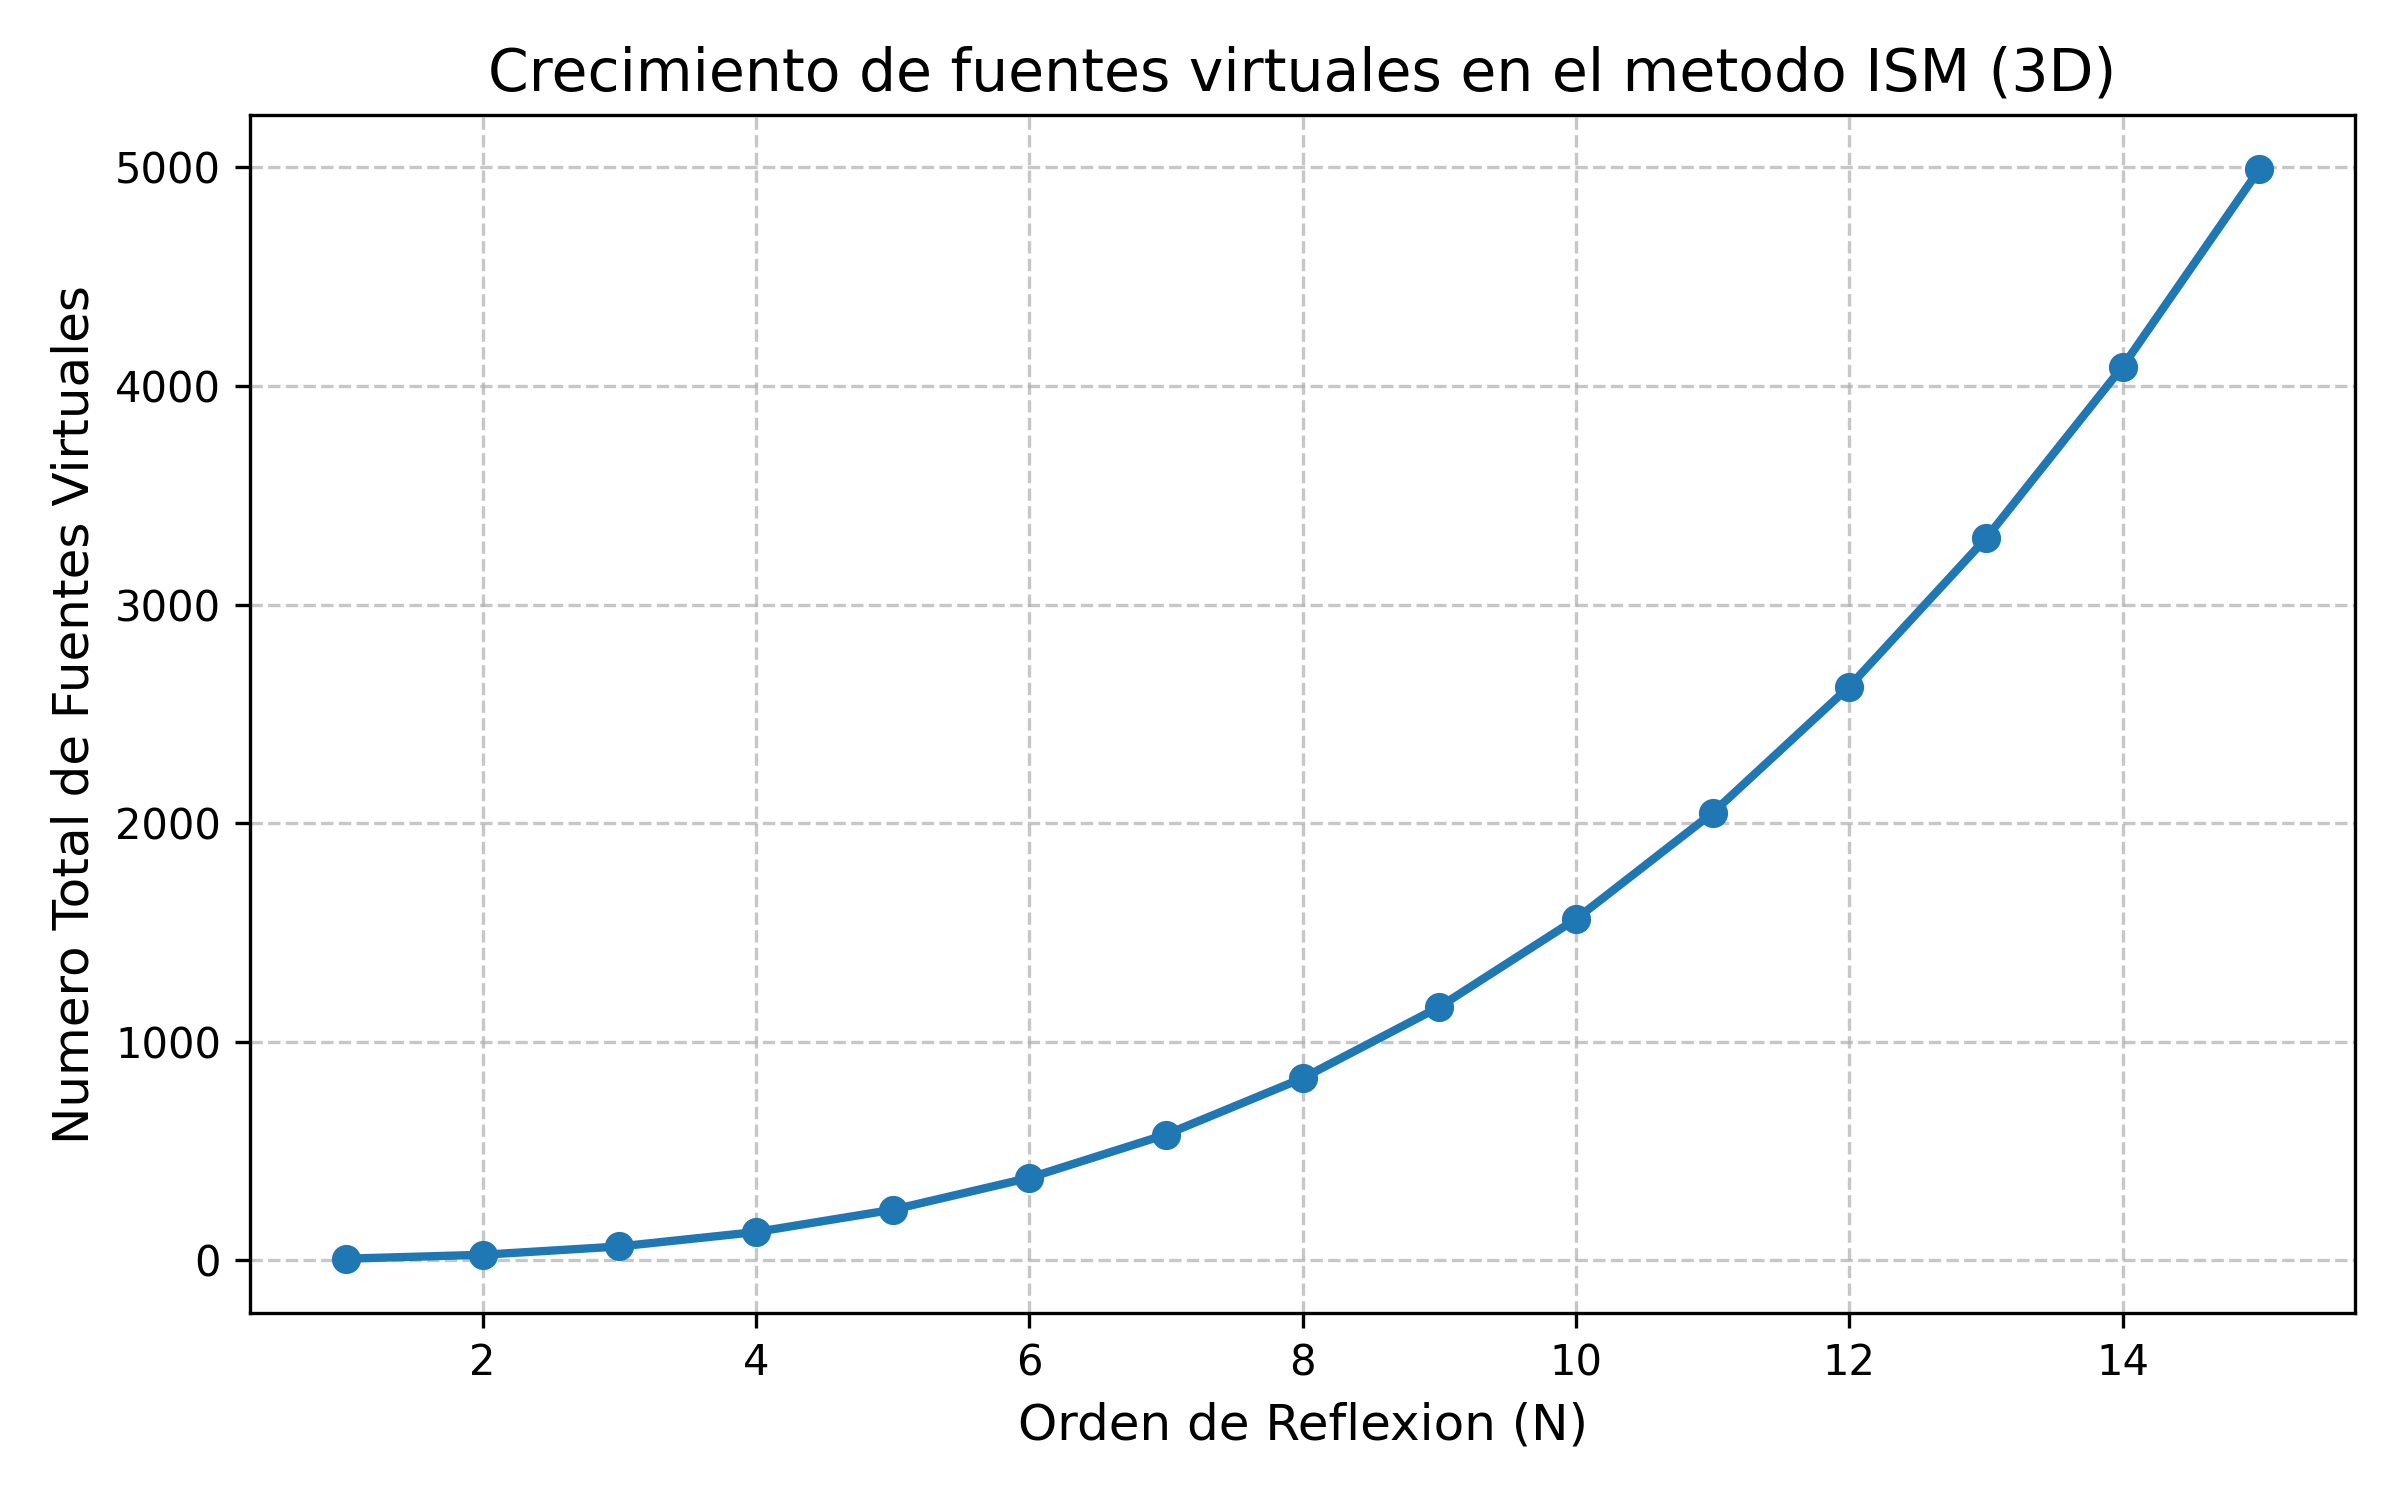
\includegraphics[width=0.8\textwidth]{../Figures/ism_cubic_growth.png}
\caption[Crecimiento cúbico en ISM]{Crecimiento del número de fuentes virtuales en el Método de Fuentes Imagen (ISM) en 3D en función del orden de reflexión $N$. La tendencia muestra un comportamiento polinómico dominante de orden cúbico, coherente con $\mathcal{O}(N^3)$.}
\label{fig:ism_cubic_growth}
\end{figure}

Este esfuerzo de cómputo se agrava drásticamente debido a la naturaleza matemática del propio método. En un espacio tridimensional, el número de fuentes virtuales generadas escala de forma \textbf{cúbica} ($O(N^3)$) con respecto al orden de reflexión $N$. Dado que la densidad de ecos en una sala real aumenta proporcionalmente al cuadrado del tiempo, simular los tramos finales de la curva de decaimiento de energía exige computar un volumen inasumible de fuentes imagen. Por tanto, mientras que el ISM es la herramienta ideal para extraer la firma geométrica inicial del recinto (los primeros milisegundos de la RIR), su crecimiento polinómico de orden tres lo descarta por completo como método autónomo para la síntesis completa de la reverberación.

\section[Aprendizaje profundo]{Enfoques basados en Machine Learning}

\subsection{De la simulación explícita a los modelos predictivos}

\subsection{FiNS: Filtered Noise Shaping}

En el ámbito de la estimación ciega de la respuesta al impulso de la sala (RIR) a partir de voz reverberante, el modelo FiNS (Filtered Noise Shaping) \cite{Steinmetz2021FiNS} propone un enfoque basado en el aprendizaje profundo para la estimación directa en el dominio del tiempo. Este método resulta útil para aplicaciones de realidad aumentada y posproducción de audio, donde se requiere un emparejamiento acústico preciso y de alta fidelidad operando a 48 kHz.

A diferencia de los enfoques que predicen parámetros para reverberadores algorítmicos o emplean modelos de transformación de gran tamaño, FiNS modela directamente la acústica del espacio basándose únicamente en una grabación de referencia. Esto permite reemplazar simulaciones complejas por una operación de convolución simple entre una señal de entrada y la RIR predicha.

Para lograr esto, la arquitectura de la red incorpora un fuerte sesgo inductivo inspirado en la acústica de salas, separando el modelado de la respuesta mediante un codificador y un decodificador especializados. El codificador en el dominio del tiempo procesa la señal de entrada utilizando bloques de convoluciones unidimensionales para capturar el comportamiento temporal a diferentes escalas, generando finalmente un espacio latente. 
   
\begin{figure}[H]
    \centering
    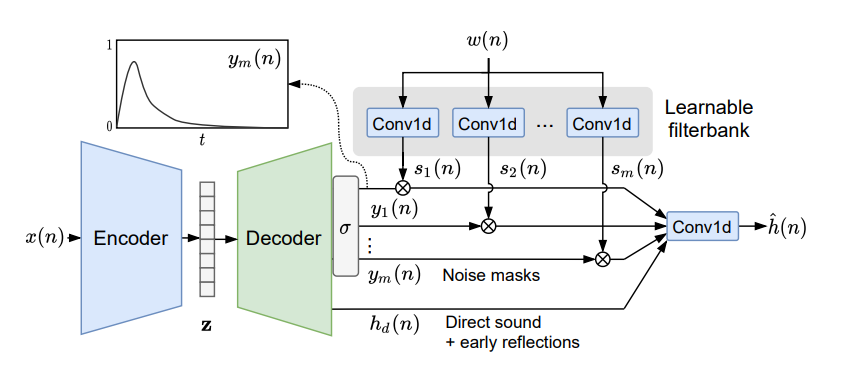
\includegraphics[width=0.8\linewidth]{Figures/arquitecture_Fins.png} % Asegúrate de guardar el recorte con este nombre
    \caption[Arquitectura de FiNS]{Esquema de la arquitectura de FiNS, destacando el codificador temporal y el decodificador especializado para modelar por separado la respuesta temprana (sonido directo y primeras reflexiones) y la reverberación tardía (cola reverberante).\cite{Steinmetz2021FiNS}}
    \label{fig:fins_architecture}
\end{figure}

En la arquitectura propuesta para la síntesis y estimación acústica, el modelo procesa una señal de entrada en el dominio del tiempo $x(n)$ mediante un codificador (\textit{Encoder}) para extraer un vector de características en el espacio latente $\mathbf{z}$. A partir de esta representación, el decodificador (\textit{Decoder}) divide la reconstrucción de la respuesta al impulso de la habitación en dos enfoques complementarios basados en la física del sonido.

Por un lado, estima de manera directa el sonido directo y las reflexiones tempranas, componente denotado como $h_d(n)$. Por otro lado, para modelar la reverberación tardía de naturaleza estocástica, el decodificador genera un conjunto de máscaras de ruido o envolventes temporales $y_1(n), \dots, y_m(n)$ (restringidas al rango de valores entre 0 y 1 mediante una función de activación sigmoide $\sigma$). 

Simultáneamente, una señal de ruido blanco continuo $w(n)$ alimenta un banco de filtros convolucionales unidimensionales entrenable (\textit{Learnable filterbank}), generando múltiples componentes de ruido en subbandas $s_1(n), \dots, s_m(n)$. Cada máscara de ruido proyectada por el decodificador modula en amplitud a su respectiva subbanda de ruido para emular el decaimiento exponencial característico de la energía acústica con el tiempo.

Finalmente, el conjunto de las subbandas moduladas por las envolventes y la componente inicial $h_d(n)$ se combinan e integran a través de una última capa convolucional de una dimensión (Conv1d) para producir la estimación completa y final de la respuesta al impulso de la habitación $\hat{h}(n)$.

El aspecto más destacable para la extrapolación acústica reside en el decodificador, el cual descompone la síntesis de la RIR modelando por separado la respuesta temprana y la cola reverberante. Por un lado, la red utiliza un canal de salida dedicado para predecir directamente en el dominio del tiempo las muestras correspondientes al sonido directo y a las primeras reflexiones.

Por otro lado, la reverberación tardía se modela como una suma de señales de ruido filtrado en decaimiento. Para generar esta cola reverberante, el decodificador produce máscaras temporales que modulan un conjunto de señales de ruido procesadas por un banco de filtros aprendibles.

Esta estrategia de combinar la predicción directa para las componentes tempranas y un enfoque estocástico basado en la conformación de ruido para la parte tardía resulta muy efectiva.

Las evaluaciones demuestran que FiNS no solo es capaz de sintetizar RIRs que coinciden con los parámetros objetivos de la sala, como el tiempo de reverberación ($T_{60}$) y la relación directo-reverberante (DRR), sino que también reproduce las características perceptivas con mayor realismo y precisión que otras arquitecturas base de aprendizaje profundo \cite{Steinmetz2021FiNS}.
\subsection[PINNs]{PINNs: Physics-Informed Neural Networks}

\subsection[DECOR]{DECOR: Deep Exponential Completion Of Room Impulse Responses}

El modelado preciso de la reverberación tardía resulta costoso computacionalmente, pero el sonido directo y las primeras reflexiones encapsulan información suficiente sobre la geometría de la sala y sus características de absorción. Para explotar esta relación, se ha formalizado la tarea de \textit{RIR completion} (completado de la respuesta al impulso de la sala), cuyo objetivo es sintetizar la reverberación tardía a partir de la porción temprana (los primeros 50~ms) de la respuesta \cite{Lin25}.

\begin{figure}[H]
    \centering
    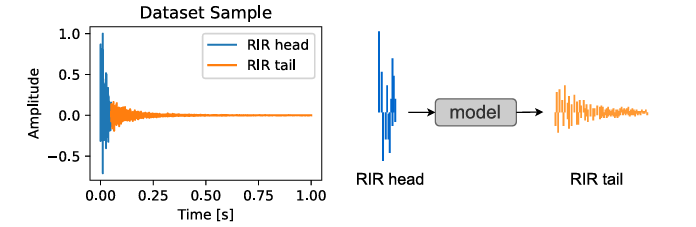
\includegraphics[width=0.68\linewidth]{Figures/rir_completion.png}
    \caption{Concepto de \textit{RIR completion}: extrapolación de la reverberación tardía a partir del tramo temprano de la respuesta al impulso \cite{Lin25}.}
    \label{fig:rir_completion}
\end{figure}


Para abordar este problema, se han propuesto arquitecturas basadas en el paradigma codificador-decodificador (\textit{encoder-decoder}). El modelo DECOR (\textit{Deep Exponential Completion Of Room impulse responses}) es un exponente de esta tendencia \cite{Lin25}. En este sistema, un codificador convolucional temporal profundo comprime la estructura de los primeros 50~ms en un vector latente de baja dimensión de 128 dimensiones. Posteriormente, un decodificador utiliza este vector para parametrizar un modelo físico de decaimiento exponencial \cite{Lin25}. 

\begin{figure}[H]
    \centering
    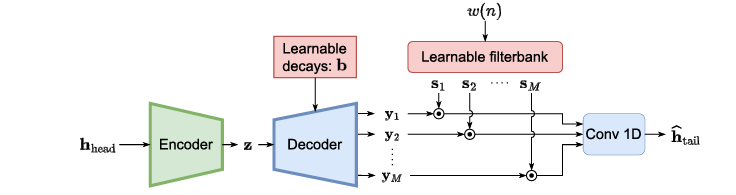
\includegraphics[width=0.75\linewidth]{Figures/encoder-decoder.png}
    \caption{Esquema general de la arquitectura DECOR. El codificador procesa la cabeza de la RIR para generar un vector latente $\mathbf{z}$, que el decodificador utiliza para predecir envolventes de decaimiento aplicadas a un banco de filtros de ruido \cite{Lin25}.}
    \label{fig:decor_overview}
\end{figure}

DECOR se presenta como una evolución conceptual y estructural frente a arquitecturas previas como FiNS (\textit{Filtered Noise Shaping}) \cite{Steinmetz2021FiNS,Lin25}. FiNS fue diseñado originalmente para una tarea de estimación ciega, tomando fragmentos de varios segundos de voz reverberante para predecir la RIR \cite{Steinmetz2021FiNS}. Aunque DECOR adapta la estructura del codificador de FiNS mediante convoluciones unidimensionales y conexiones residuales, la diferencia fundamental entre ambas redes radica en el diseño de su decodificador y en la imposición de un fuerte sesgo inductivo basado en la acústica de salas para la síntesis de la reverberación tardía \cite{Lin25}.

Mientras que el decodificador de FiNS utiliza un enfoque basado en sobremuestreo convolucional (\textit{convolution upsampling}) \cite{Steinmetz2021FiNS}, DECOR modela estocásticamente la reverberación tardía como ruido blanco moldeado por una suma de envolventes de decaimiento exponencial \cite{Lin25}. Específicamente, el decodificador de DECOR emplea un perceptrón multicapa (MLP) que toma el vector latente y predice matrices de amplitud temporal. Estas amplitudes se multiplican por tasas de decaimiento aprendibles (inicializadas para decaimientos $T_{60}$ entre 0.05 y 3.0 segundos) para formar envolventes que modulan secuencias de ruido generadas por un banco de filtros de respuesta finita (FIR) en bandas de octava \cite{Lin25}.

Esta reformulación arquitectónica aporta ventajas significativas frente a FiNS que justifican su adopción para el completado de RIRs:

\begin{itemize}
    \item \textbf{Eficiencia computacional y tamaño del modelo:} La parametrización física en el decodificador permite que DECOR sea extremadamente ligero. El modelo DECOR ocupa únicamente 37~MB, lo que lo hace más de 30 veces más pequeño que la arquitectura base de FiNS, cuyo peso asciende a 1,3~GB \cite{Lin25}. Esta reducción drástica de parámetros facilita su despliegue en aplicaciones de síntesis en tiempo real para entornos dinámicos de realidad virtual o aumentada.
    
    \item \textbf{Eliminación de artefactos acústicos:} Las redes generativas que no imponen restricciones físicas estrictas sobre la síntesis de la señal suelen presentar problemas perceptuales. FiNS tiende a generar picos dispersos de gran amplitud en la cola de la RIR, lo que introduce una "granulosidad" (\textit{graininess}) poco natural en el audio resultante \cite{Steinmetz2021FiNS,Lin25}. Al forzar a la red a predecir parámetros para un modelo de decaimiento exponencial puro, DECOR garantiza curvas de decaimiento suaves y un sonido más realista y coherente con el comportamiento acústico natural \cite{Lin25}.
    
    \item \textbf{Mejora en métricas objetivas:} DECOR supera a FiNS en la evaluación de la similitud con las características acústicas de la sala objetivo. Logra reducir el error en el dominio espectro-temporal (MSTFT), mejora la precisión de la función de decaimiento de energía (EDF), y estima con mayor exactitud tanto el tiempo de reverberación ($T_{60}$) como la relación directo-reverberante (DRR) \cite{Lin25}. 
    
    \item \textbf{Capacidad de generalización:} Aunque la extrapolación de una señal a veinte veces su longitud original es una tarea compleja que penaliza a ambos modelos ante datos no vistos, DECOR mantiene un mejor rendimiento de generalización. Frente a conjuntos de datos de medición reales que la red no ha observado durante el entrenamiento, DECOR sigue siendo capaz de deducir relaciones correctas del $T_{60}$ y superar a FiNS, demostrando que su arquitectura de decaimiento estructurado es más robusta frente a escenarios acústicos fuera de distribución \cite{Lin25}.
\end{itemize}

En conclusión, la transición de un enfoque de sobremuestreo genérico a un modelo fuertemente condicionado por la física acústica permite que DECOR resuelva el problema del \textit{RIR completion} de forma mucho más eficiente. La parametrización directa de variables como el decaimiento por bandas de octava no solo elimina la inestabilidad de las muestras individuales, sino que dota a la red de una alta expresividad para modelar escenarios acústicos complejos manteniendo una huella computacional mínima. Por este motivo, DECOR constituye el método seleccionado para ser implementado y empleado en el desarrollo de este trabajo.

